\section{Modelling Our Climate}
\label{sec:climate-modelling}

Throughout the previous sections, we have discussed a number of climate models
with varying levels of complexity. They are all based on the fundamental
principle of energy conservation and equillibrium, i.e. energy input = energy
output for a planet in equillibrium, known as energy balance models (\gls{EBM}).
In this section we will have a look at some
of these models and explore different ways in which we can apply this principle 
to make more nuanced models.

\subsection{Energy Balance Models}
\label{sec:EBM}

\subsubsection{The Zero and One-Dimensional Energy Balance Models}
\label{sec:0D-1D-EBM}

The simplest energy balance model is the zero-dimensional energy balance model. 
We have covered this extensively in sections \ref{sec:introduction} and 
\ref{greenhouse_effect}. It is the model of photon energy exchange where the Earth
gets all its energy from the Sun and radiates it back into space (through albedo,
blackbody radiation etc.). 

Within this model we explored the \textbf{zero-layer} version, i.e. the no-atmosphere
model where we only account for the energy coming from the sun, 
\hyperlink{glo:albedo}{albedo} and blackbody radiation from the Earth's surface.
This was the energy balance equation:
$$
(1-\alpha) \text{\hyperlink{glo:TSI}{TSI}} = \sigma T_s^4
$$

Also in the aforementioned lectures is the \textbf{one-layer} version, i.e. the
atmosphere is treated as a single layer. In such a model we also account for the
\hyperlink{glo:emissivity}{emissivity} of the atmosphere and its 
\hyperlink{glo:absorptivity}{absorptivity} (which we stated are
equal in value for a system in \gls{LTE}). This was the energy balance equation:
$$
(1-\alpha) \text{\hyperlink{glo:TSI}{TSI}} = (1-\epsilon_a)\sigma T_s^4 + 
\epsilon_a\sigma T_a^4
$$
and it also lead to the introduction of the greenhouse effect. For more details 
see section \ref{greenhouse_effect}.\\

We can now extend this model to make it what is known as the \textbf{1-D \gls{EBM}}.
In this model we introduce latidudinal dependence. This is an obvious first choice
for independent variable since it is apparent that the energy balance is going 
to be different in the poles than in the equator.\footnote{We could also add
time-dependency, since it is apparent that this also has a significant effect}.
For now we will only consider the mean anual values for the energy balance, see
figure \ref{fig:1D-EBM}.

\begin{figure}[h]
    \centering
    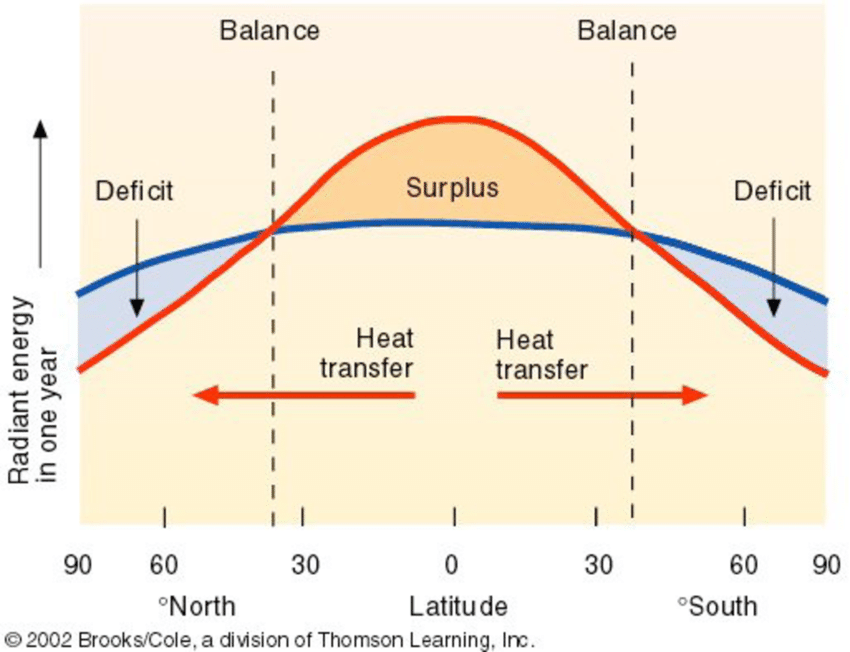
\includegraphics[width=0.6\textwidth]{figures/1debm.png}
    \caption{The 1-D Energy Balance Model. The energy balance is different in the
    poles than in the equator.}
    \label{fig:1D-EBM}
\end{figure}

As we see in figure \ref{fig:1D-EBM}, the energy balance is different in the
poles than it is in the equator (when averaged over the year). The relevance of 
this is that this will set the main circulation patterns of energy (both 
atmospheric and oceanic).

Let's express this model mathematically. We begin by writing the energy balance
equation:
$$
\frac{(1-\alpha)}{4} \text{\hyperlink{glo:TSI}{TSI}} = \epsilon'\sigma T_s^4
$$
where $\epsilon'$ is the effective emissivity of the Earth (see
\ref{sec:decompose_feedback}). It follows that for a perturbation from equillibrium
$$
C \frac{dT_s}{dt} = \frac{(1-\alpha)}{4} \text{\hyperlink{glo:TSI}{TSI}} - 
\epsilon'\sigma T_s^4
$$
where $C$ is the heat capacity per square meter. For a short range of values for
$T_s$ we can linearise as follows and substitute into the equation:
$$
\epsilon' \sigma T_s^4 \approx A + BT_s \quad \implies \quad C \frac{dT_s}{dt} 
\approx \frac{(1-\alpha)}{4} \text{\hyperlink{glo:TSI}{TSI}} - (A + BT_s)
$$
where $A$ and $B$ are constants. We can now ``slice'' the Earth into small 
latitudinal bands and consider the energy balance in each band $i$:
$$
C_i \frac{dT_{s,i}}{dt} \approx \frac{(1-\alpha_i)}{4} 
\text{\hyperlink{glo:TSI}{TSI}}_i - A - BT_{s,i}
$$
and finally we can include a term for the lateral heat transport ($F$) to complete
the model:
$$
C_i \frac{dT_{s,i}}{dt} + F(T_{s, i} - T_s) \approx \frac{(1-\alpha_i)}{4} 
\text{\hyperlink{glo:TSI}{TSI}}_i - A - BT_{s,i}
$$
where $F$ is in units of $Wm^{-2}K^{-1}$. The one-dimensional energy balance
model \textbf{must be solved numerically}.

\begin{figure}[h]
    \centering
    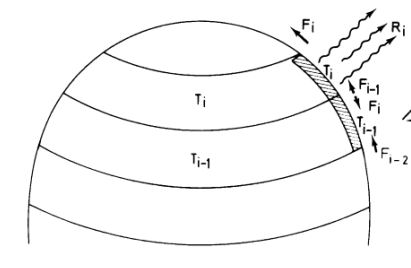
\includegraphics[width=0.4\textwidth]{figures/1demb diagram.png}
    \caption{Diagram of the 1D EMB.}
    \label{fig:1D-EBM-diagram}
\end{figure}

\subsubsection{Coupled General Circulation Models (CGCMs)}
\label{sec:CGCMs}

These are the most complex and complete models available, so called ``state-of-the-art''.
These are the kind of models used by the IPCC to make predictions about the future.
In the course we do not go too much into detail about these models, precisely due
to their complexity.\\

In these models, both the atmosphere and the ocean are divided into a grid of
boxes. The atmosphere is further divided into layers of altitude. These systems
are modelled as a set of coupled non-linear ordinary differential equations that
govern the evolution of the systems from a fluid dynamics perspective (in the 
atmosphere and ocean) while always ensuring conservation of momentum, mass and
energy.

Models have evolved significantly over time, with more and more layers of complexity
being added as computing power available increases and new inter-dependencies 
within the climate system are identified (i.e. the science evolves). Figure
\ref{fig:evolution-cgcm} shows the evolution of CGCMs over time with more components
being added as time goes on.

\begin{figure}[h]
    \centering
    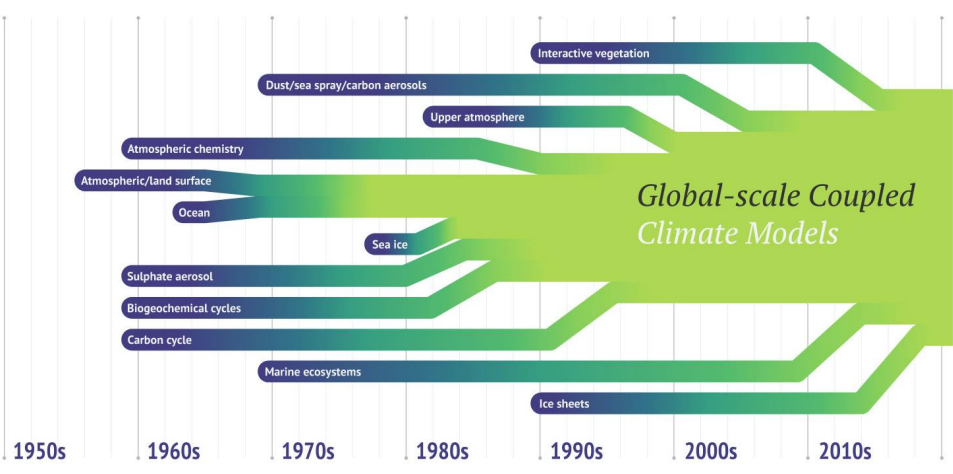
\includegraphics[width=0.75\textwidth]{figures/evolution cgcm.png}
    \caption{Evolution of CGCMs over time.}
    \label{fig:evolution-cgcm}
\end{figure}

\subsubsection{Earth System Models}
\label{sec:ESMs}

These are the absolute most advanced models available. They are essentially CGCMs
but not only simulate physical processes (oceans, land, atmosphere) but also
biogeochemical processes (most notably the carbon cycle) and the way they interact
with each other. This allows to introduce some additional feedbacks into the model
that are not present in CGCMs such as how warming may affect the ability of forests 
to absorb \ce{CO2}, or how changes in ocean circulation may alter the ocean's 
\ce{CO2} uptake.

\subsection{Model Parametrisation}
\label{sec:model-parametrisation}

In climate modelling, certain physical process cannot be modelled in a per-cell
basis due to their scale being too small, e.g. convection, cloud formation and
evolution and others. To model these, we use \textbf{parametrisation}.\\

In parametrisation, we find simplified 
representations or approximations of sub-grid phenomena, expressed in terms
of the larger-scale variables that the model does directly resolve. They are 
often based on empirical evidence from observations or more detailed process-based 
studies, or on theoretical understanding from physical laws. Within parametrisation
techniques we find two main types:\\

\textbf{Diagnostic Scheme}: A diagnostic scheme determines the outcome (e.g., 
the presence and properties of clouds) directly from the current state of the 
large-scale variables, with no memory of past states. In other words, given the 
same current state, a diagnostic scheme will always produce the same outcome.\\

\textbf{Prognostic Scheme}: A prognostic scheme is more advanced, it includes some 
form of temporal evolution or memory, meaning that the outcome can depend on past 
states as well as the current state. This allows the model to represent processes 
that have some inherent time-dependence or persistence, such as the life cycle of 
clouds or the accumulation of snow. Given the same current state, a prognostic 
scheme could produce different outcomes depending on the prior sequence of states.\\

\noindent The main idea to remember between the two is that prognostic schemes
have memory (time dependence) while diagnostic schemes do not.

Also worth remembering is that clouds are the main source of uncertainty in climate
models by far, analytical solutions become impossible so with every approximation
comes error (error in frequency of occurrence, error in amount and properties and
error in location and timing).

\subsection{Costs of Climate Modelling}
\label{sec:costs-climate-modelling}

Climate models are very expensive to run, both in terms of computing power and
time.
\begin{itemize}
    \item Atmosphere is the most expensive component of the model to run and is
    typically the bottle neck of climate models (radiation and chemistry schemes
    are very computationally intensive)
    \item Timestep in Earth System Model worlds is typically 20 minutes for
    dynamics and 1h for radiation
    \item 1 week of very high performance computer time yields about 40 years of
    simulated climate. When we consider that we want to simulate 1000 or 2000 years
    of climate per model, and include many of them in an ensemble for an IPCC report
    we can see how this becomes a very expensive and time consuming process.
    \item There is about 1 million `basic' variables only to model oceans and
    atmosphere. This is very memory consuming
\end{itemize}

